 \chapter{Funções}

\section{Definição de funções}

\vskip0.3cm
 \colorbox{azul}{
 \begin{minipage}{0.9\linewidth}
 \begin{center}
  Dados dois conjuntos $A$ e $B$ não vazios, de números Reais, ou seja, $A \subseteq \mathbb{R}$ e $B \subseteq \mathbb{R}$. Uma \textbf{aplicação} de $A$ em $B$ ou \textbf{função} definida no conjunto $A$ com imagens em $B$ é uma regra (equação) que diz como associar cada elemento $x \in A$ a um \underline{único} $y \in B$.
 \end{center}
 \end{minipage}}
 \vskip0.3cm


 Exemplos de relações que são funções de $A$ em $B$:
 \begin{multicols}{3}
 \begin{tikzpicture}
 \node (1) at (0,0) {1};%\filldraw(1.east) circle (1pt)
 \node (2) [below of=1] {2};%\filldraw(2.east) circle (1pt)
 \node (3) [below of=2] {3};%\filldraw(3.east) circle (1pt)
 \node[fit=(1) (2) (3),ellipse,draw=red,minimum width=1cm,thick,label=below:\(A\)]{};

 \node (a) at (3,0) {a};%\filldraw($b_1$.west) circle (1pt)
 \node (b) [below of=a] {b};%\filldraw($b_2$.west) circle (1pt)
 \node (c) [below of=b] {c};%\filldraw($b_3$.west) circle (1pt)
 \node[fit=(a) (b) (c),ellipse,draw=green,minimum width=1cm,thick,label=below:\(B\)]{};

 \draw[->, shorten >=.1cm, >=stealth'] (1.east) to (a.west);
 \draw[->, shorten >=.1cm, >=stealth'] (2.east) to (b.west);
 \draw[->, shorten >=.1cm, >=stealth'] (3.east) to (c.west);
\end{tikzpicture} \\
 \begin{tikzpicture}
 \node (1) at (0,0) {1};%\filldraw(1.east) circle (1pt)
 \node (2) [below of=1] {2};%\filldraw(2.east) circle (1pt)
 \node (3) [below of=2] {3};%\filldraw(3.east) circle (1pt)
 \node[fit=(1) (2) (3),ellipse,draw=red,minimum width=1cm,thick,label=below:\(A\)]{};

 \node (a) at (3,0) {a};%\filldraw($b_1$.west) circle (1pt)
 \node (b) [below of=a] {b};%\filldraw($b_2$.west) circle (1pt)
 \node (c) [below of=b] {c};%\filldraw($b_3$.west) circle (1pt)
 \node[fit=(a) (b) (c),ellipse,draw=green,minimum width=1cm,thick,label=below:\(B\)]{};

 \draw[->, shorten >=.1cm, >=stealth'] (1.east) to (a.west);
 \draw[->, shorten >=.1cm, >=stealth'] (2.east) to (a.west);
 \draw[->, shorten >=.1cm, >=stealth'] (3.east) to (c.west);
\end{tikzpicture} \\
\begin{tikzpicture}
 \node (1) at (0,0) {1};%\filldraw(1.east) circle (1pt)
 \node (2) [below of=1] {2};%\filldraw(2.east) circle (1pt)
 \node (3) [below of=2] {3};%\filldraw(3.east) circle (1pt)
 \node[fit=(1) (2) (3),ellipse,draw=red,minimum width=1cm,thick,label=below:\(A\)]{};

 \node (a) at (3,0) {a};%\filldraw($b_1$.west) circle (1pt)
 \node (b) [below of=a] {b};%\filldraw($b_2$.west) circle (1pt)
 \node (c) [below of=b] {c};%\filldraw($b_3$.west) circle (1pt)
 \node[fit=(a) (b) (c),ellipse,draw=green,minimum width=1cm,thick,label=below:\(B\)]{};

 \draw[->, shorten >=.1cm, >=stealth'] (1.east) to (b.west);
 \draw[->, shorten >=.1cm, >=stealth'] (2.east) to (b.west);
 \draw[->, shorten >=.1cm, >=stealth'] (3.east) to (b.west);
\end{tikzpicture}

\end{multicols}



 Exemplos de relações que não são funções de $A$ em $B$:
\begin{multicols}{3}
\begin{tikzpicture}
 \node (1) at (0,0) {1};%\filldraw(1.east) circle (1pt)
 \node (2) [below of=1] {2};%\filldraw(2.east) circle (1pt)
 \node (3) [below of=2] {3};%\filldraw(3.east) circle (1pt)
 \node[fit=(1) (2) (3),ellipse,draw=red,minimum width=1cm,thick,label=below:\(A\)]{};

 \node (a) at (3,0) {a};%\filldraw($b_1$.west) circle (1pt)
 \node (b) [below of=a] {b};%\filldraw($b_2$.west) circle (1pt)
 \node (c) [below of=b] {c};%\filldraw($b_3$.west) circle (1pt)
 \node[fit=(a) (b) (c),ellipse,draw=green,minimum width=1cm,thick,label=below:\(B\)]{};

 \draw[->, shorten >=.1cm, >=stealth'] (1.east) to (a.west);
 \draw[->, shorten >=.1cm, >=stealth'] (1.east) to (b.west);
 \draw[->, shorten >=.1cm, >=stealth'] (2.east) to (b.west);
 \draw[->, shorten >=.1cm, >=stealth'] (3.east) to (c.west);
\end{tikzpicture} \\
\begin{tikzpicture}
 \node (1) at (0,0) {1};%\filldraw(1.east) circle (1pt)
 \node (2) [below of=1] {2};%\filldraw(2.east) circle (1pt)
 \node (3) [below of=2] {3};%\filldraw(3.east) circle (1pt)
 \node[fit=(1) (2) (3),ellipse,draw=red,minimum width=1cm,thick,label=below:\(A\)]{};

 \node (a) at (3,0) {a};%\filldraw($b_1$.west) circle (1pt)
 \node (b) [below of=a] {b};%\filldraw($b_2$.west) circle (1pt)
 \node (c) [below of=b] {c};%\filldraw($b_3$.west) circle (1pt)
 \node[fit=(a) (b) (c),ellipse,draw=green,minimum width=1cm,thick,label=below:\(B\)]{};

 \draw[->, shorten >=.1cm, >=stealth'] (1.east) to (a.west);
 %\draw[->, shorten >=.1cm, >=stealth'] (2.east) to (b.west);
 \draw[->, shorten >=.1cm, >=stealth'] (3.east) to (c.west);
\end{tikzpicture} \\
\begin{tikzpicture}
 \node (1) at (0,0) {1};%\filldraw(1.east) circle (1pt)
 \node (2) [below of=1] {2};%\filldraw(2.east) circle (1pt)
 \node (3) [below of=2] {3};%\filldraw(3.east) circle (1pt)
 \node[fit=(1) (2) (3),ellipse,draw=red,minimum width=1cm,thick,label=below:\(A\)]{};

 \node (a) at (3,0) {a};%\filldraw($b_1$.west) circle (1pt)
 \node (b) [below of=a] {b};%\filldraw($b_2$.west) circle (1pt)
 \node (c) [below of=b] {c};%\filldraw($b_3$.west) circle (1pt)
 \node[fit=(a) (b) (c),ellipse,draw=green,minimum width=1cm,thick,label=below:\(B\)]{};

 \draw[->, shorten >=.1cm, >=stealth'] (1.east) to (a.west);
 \draw[->, shorten >=.1cm, >=stealth'] (1.east) to (b.west);
 %\draw[->, shorten >=.1cm, >=stealth'] (2.east) to (b.west);
 \draw[->, shorten >=.1cm, >=stealth'] (3.east) to (c.west);
\end{tikzpicture}
\end{multicols}

\newpage

Usamos normalmente a seguinte notação:
\[f: A \rightarrow B\]
que se lê: $f$ é uma função de $A$ em $B$.

A função $f$ transforma $x \in A$ em $y \in B$. Denotamos isso da seguinte forma:
\[f(x) = y .\]

Simplificando as notações podemos representar as duas informações acima da seguinte forma:
\begin{eqnarray*}
 f: A & \rightarrow & B \\
 x & \mapsto & y.
\end{eqnarray*}

Dada uma função $f: A \rightarrow B$, o conjunto $A$ chama-se \textbf{domínio} da função $f$ e o conjunto $B$ chama-se \textbf{contradomínio} da função $f$.  Para cada $x \in A$, o elemento $f(x)= y \in B$ chama-se imagem de $x$ pela função $f$. Assim o conjunto \textbf{imagem} da função $f$ é dado por:
\[Im(f)= \{ y \in B \mid y = f(x) \text{ para algum } x \in A\} .\]

Em outras palavras o domínio de uma função é um subconjunto de números Reais nos quais faz sentido aplicar a regra da função, e contradomínio é o conjunto $\mathbb{R}$, ou um subconjunto de $\mathbb{R}$ que contenha o conjunto $Im(f)$.

E o \textbf{gráfico} da função é dado por:
\[Gr(f) = \{ (x, y) \in A \times B \mid x \in A, y = f(x) \in B\} .\]

\begin{exem}
 Considere os conjuntos $A= \{1, 2, 3\}$ e $B= \{a, b, c, d\}$ e a regra de relação entre estes dois conjuntos dada pelo diagrama abaixo,

 \begin{figure}[H]
 \centering
 \begin{tikzpicture}
 \node (1) at (0,0) {1};%\filldraw(1.east) circle (1pt)
 \node (2) [below of=1] {2};%\filldraw(2.east) circle (1pt)
 \node (3) [below of=2] {3};%\filldraw(3.east) circle (1pt)
 \node[fit=(1) (2) (3),ellipse,draw=red,minimum width=1cm,thick,label=below:\(A\)]{};

 \node (a) at (3,0) {a};%\filldraw($b_1$.west) circle (1pt)
 \node (b) [below of=a] {b};%\filldraw($b_2$.west) circle (1pt)
 \node (c) [below of=b] {c};%\filldraw($b_3$.west) circle (1pt)
 \node (d) [below of=c] {d};%\filldraw($b_3$.west) circle (1pt)
 \node[fit=(a) (b) (c) (d),ellipse,draw=green,minimum width=1cm,thick,label=below:\(B\)]{};

 \draw[->, shorten >=.1cm, >=stealth'] (1.east) to (b.west);
 \draw[->, shorten >=.1cm, >=stealth'] (2.east) to (c.west);
 \draw[->, shorten >=.1cm, >=stealth'] (3.east) to (a.west);
\end{tikzpicture}
\end{figure}
note que esta regra define uma função $f: A \rightarrow B$, cujo domínio é $Dom(f) = A$, contra-domínio é $CDom(f) = B$, e a imagem é $Im(f)= \{a, b, c\}$, observe que $Im(f) \subset CDom(f)$. Pela definição temos que o gráfico da $f$ será o conjunto $Gr(f)= \{(1, b); (2, c); (3, a)\}$ que pode ser representado geometricamente como feito na figura abaixo:

\begin{figure}[H]
 \centering
    \fbox{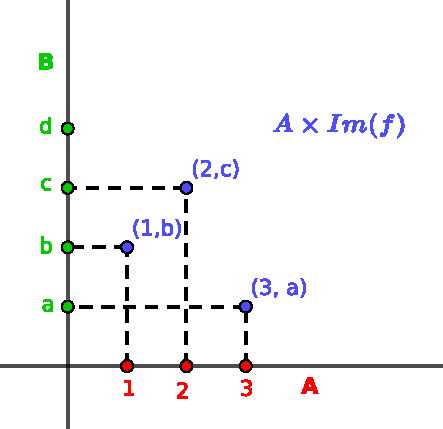
\includegraphics[width=7cm]{../Topicos/Figuras/Grf.pdf}}
    \caption{Gráfico da função $f$}
  \end{figure}

\end{exem}


\subsection{Propriedades}
As funções são classificadas em:

\begin{itemize}
 \item \textbf{Injetora}

 Uma função $f: A \rightarrow B$ é injetiva, ou injetora quando:
 \[ x_1 \neq x_2 \in A \Rightarrow f(x_1) \neq f(x_2) \in B ,\]
 ou equivalentemente usando a contrapositiva:
 \[f(x_1) = f(x_2) \in B \Rightarrow x_1 = x_2 .\]
 Ou seja, quando cada elemento da $Im(f)$ recebe um único elemento de $A= Dom(f)$, neste caso pode ocorrer de alguns elementos de $B$ não serem imagem de nenhum elemento de $A$ pela função $f$.

 \item \textbf{Sobrejetora}

 Uma função $f: A \rightarrow B$ é sobrejetiva, ou sobrejetora quando para todo $y \in B$, existe pelo menos um elemento $x \in A$ tal que $f(x) = y$. Equivalentemente em símbolos:
 $$\forall y \in B, \exists x \in A \text{ tal que } f(x) = y$$
 Ou ainda, quando cada elemento de $B$ recebe algum elemento de $A$, neste caso podendo não ser único.

 \item \textbf{Bijetora}

 Uma função $f: A \rightarrow B$ é bijetora, ou bijetiva quando for simultaneamente injetora e sobrejetora. Neste caso, $f$ admite uma inversa que é denotada por $f^{(-1)}$.

\end{itemize}

\begin{multicols}{2}
 \begin{tikzpicture}
 \node (1) at (0,0) {1};%\filldraw(1.east) circle (1pt)
 \node (2) [below of=1] {2};%\filldraw(2.east) circle (1pt)
 \node (3) [below of=2] {3};%\filldraw(3.east) circle (1pt)
 \node[fit=(1) (2) (3),ellipse,draw=red,minimum width=1cm,thick,label=below:\(A\)]{};

 \node (a) at (3,0) {a};%\filldraw($b_1$.west) circle (1pt)
 \node (b) [below of=a] {b};%\filldraw($b_2$.west) circle (1pt)
 \node (c) [below of=b] {c};%\filldraw($b_3$.west) circle (1pt)
 \node[fit=(a) (b) (c),ellipse,draw=green,minimum width=1cm,thick,label=below:\(B\)]{};

 \draw[->, shorten >=.1cm, >=stealth'] (1.east) to (c.west);
 \draw[->, shorten >=.1cm, >=stealth'] (2.east) to (b.west);
 \draw[->, shorten >=.1cm, >=stealth'] (3.east) to (a.west);
\end{tikzpicture} \\
 \textbf{bijetora}\\
 \begin{tikzpicture}
 \node (1) at (0,0) {1};%\filldraw(1.east) circle (1pt)
 \node (2) [below of=1] {2};%\filldraw(2.east) circle (1pt)
 \node (3) [below of=2] {3};%\filldraw(3.east) circle (1pt)
 \node[fit=(1) (2) (3),ellipse,draw=red,minimum width=1cm,thick,label=below:\(A\)]{};

 \node (a) at (3,0) {a};%\filldraw($b_1$.west) circle (1pt)
 \node (b) [below of=a] {b};%\filldraw($b_2$.west) circle (1pt)
 \node[fit=(a) (b),ellipse,draw=green,minimum width=1cm,thick,label=below:\(B\)]{};

 \draw[->, shorten >=.1cm, >=stealth'] (1.east) to (a.west);
 \draw[->, shorten >=.1cm, >=stealth'] (2.east) to (a.west);
 \draw[->, shorten >=.1cm, >=stealth'] (3.east) to (b.west);
\end{tikzpicture} \\
\textbf{sobrejetora \\ e \\ não injetora}
\end{multicols}

\begin{multicols}{2}
 \begin{tikzpicture}
 \node (1) at (0,0) {1};%\filldraw(1.east) circle (1pt)
 \node (2) [below of=1] {2};%\filldraw(2.east) circle (1pt)
 \node (3) [below of=2] {3};%\filldraw(3.east) circle (1pt)
 \node[fit=(1) (2) (3),ellipse,draw=red,minimum width=1cm,thick,label=below:\(A\)]{};

 \node (a) at (3,0) {a};%\filldraw($b_1$.west) circle (1pt)
 \node (b) [below of=a] {b};%\filldraw($b_2$.west) circle (1pt)
 \node (c) [below of=b] {c};%\filldraw($b_3$.west) circle (1pt)
 \node[fit=(a) (b) (c),ellipse,draw=green,minimum width=1cm,thick,label=below:\(B\)]{};

 \draw[->, shorten >=.1cm, >=stealth'] (1.east) to (b.west);
 \draw[->, shorten >=.1cm, >=stealth'] (2.east) to (b.west);
 \draw[->, shorten >=.1cm, >=stealth'] (3.east) to (a.west);
\end{tikzpicture} \\
\textbf{não sobrejetora \\ e \\ não injetora}\\
 \begin{tikzpicture}
 \node (1) at (0,0) {1};%\filldraw(1.east) circle (1pt)
 \node (2) [below of=1] {2};%\filldraw(2.east) circle (1pt)
 \node (3) [below of=2] {3};%\filldraw(3.east) circle (1pt)
 \node[fit=(1) (2) (3),ellipse,draw=red,minimum width=1cm,thick,label=below:\(A\)]{};

 \node (a) at (3,0) {a};%\filldraw($b_1$.west) circle (1pt)
 \node (b) [below of=a] {b};%\filldraw($b_2$.west) circle (1pt)
 \node (c) [below of=b] {c};%\filldraw($b_3$.west) circle (1pt)
 \node (d) [below of=c] {d};%\filldraw($b_3$.west) circle (1pt)
 \node[fit=(a) (b) (c) (d),ellipse,draw=green,minimum width=1cm,thick,label=below:\(B\)]{};

 \draw[->, shorten >=.1cm, >=stealth'] (1.east) to (b.west);
 \draw[->, shorten >=.1cm, >=stealth'] (2.east) to (c.west);
 \draw[->, shorten >=.1cm, >=stealth'] (3.east) to (a.west);
\end{tikzpicture} \\
\textbf{não sobrejetora \\ e \\ injetora}
\end{multicols}

\begin{exem}

 \begin{enumerate}
  \item $f: \mathbb{R} \rightarrow \mathbb{R}$ tal que $f(x) = x^2$

  Neste caso, $f$ não é sobrejetora, nem injetora.

  \begin{dem}

   \begin{itemize}
    \item Sobrejetora

    $f$ não é sobrejetora porque $x^2 \geq 0$, $\forall x \in \mathbb{R}$, logo se considerarmos $y < 0 \in \mathbb{R}$ teremos que $\nexists x \in \mathbb{R}$ tal que $f(x)= y$. Portanto $f$ não é sobrejetora.
    \fim
    \item Injetora

     Note que $ \forall x \in \mathbb{R} \Rightarrow -x \in \mathbb{R}$ e que
    \[f(-x)= (-x)^2 = (-x)*(-x) = (x)*(x) = x^2 = f(x)\]
    o que mostra que $f$ não é injetora.

   \end{itemize}
  \end{dem}

  \item $f: \mathbb{R_{+}} \rightarrow \mathbb{R}$ tal que $f(x) = x^2$

  Neste caso, $f$ não é sobrejetora, mas é injetora.

  \begin{dem}
   \begin{itemize}
    \item Sobrejetora

    $f$ não é sobrejetora porque $x^2 \geq 0$, $\forall x \in \mathbb{R}$, logo se considerarmos $y < 0 \in \mathbb{R}$ teremos que $\nexists x \in \mathbb{R}$ tal que $f(x)= y$. Portanto $f$ não é sobrejetora.
    \fim
    \item Injetora

    Tome $x_1=x_2 \in \mathbb{R_{+}}$ qualquer, como
    \[x_1=x_2 \Rightarrow x_1^2=x_2^2 \Rightarrow f(x_1)=f(x_2)\]
    logo $f$ é injetora.

   \end{itemize}
  \end{dem}

  \item $f: \mathbb{R} \rightarrow \mathbb{R_{+}}$ tal que $f(x) = x^2$

  Neste caso, $f$ é sobrejetora, mas não é injetora.

  \begin{dem}
   \begin{itemize}
    \item Sobrejetora

    Tome $y \in \mathbb{R_{+}}$ qualquer, como $y \geq 0$ existe $x \in \mathbb{R}$ tal que
    \[x = \sqrt{y} \Rightarrow x^2 = (\sqrt{y})^2 \Rightarrow x^2 = y \Rightarrow f(x) = y \]
    portanto $f$ é sobrejetora.
    \fim
    \item Injetora

    Note que $ \forall x \in \mathbb{R} \Rightarrow -x \in \mathbb{R}$ e que
    \[f(-x)= (-x)^2 = (-x)*(-x) = (x)*(x) = x^2 = f(x)\]
    o que mostra que $f$ não é injetora.

   \end{itemize}
  \end{dem}

  \item $f: \mathbb{R_{+}} \rightarrow \mathbb{R_{+}}$ tal que $f(x) = x^2$ ou $f: \mathbb{R_{-}} \rightarrow \mathbb{R_{+}}$ tal que $f(x) = x^2$

  Neste caso, $f$ é sobrejetora, e é injetora, portanto bijetora.

  \begin{dem}
   \begin{itemize}
    \item Sobrejetora

    Tome $y \in \mathbb{R_{+}}$ qualquer, como $y \geq 0$ existe $x \in \mathbb{R}$ tal que
    \[x = \sqrt{y} \Rightarrow x^2 = (\sqrt{y})^2 \Rightarrow x^2 = y \Rightarrow f(x) = y\]
    portanto $f$ é sobrejetora.
    \fim
    \item Injetora

    Tome $x_1, x_2 \in \R_{+}$, tais que $f(x_1) = f(x_2)$ logo,
    \[f(x_1) = f(x_2) \Rightarrow x_1^2= x_2^2 \Rightarrow \sqrt{x_1^2}= \sqrt{x_2^2} \Rightarrow |x_1|= |x_2| \Rightarrow x_1= x_2, \]
    pois $x_1, x_2 \geqslant 0$. Portanto $f$ é injetora.

   \end{itemize}
  \end{dem}

 \end{enumerate}

\end{exem}

\subsection{Operações com funções}
Dadas as funções $f: A \rightarrow \R$, $g: B \rightarrow \R$, se $A \cap B \neq \emptyset$, então $\forall x \in A \cap B$, definimos as seguintes operações entre estas funções:
\[(f + g)(x)= f(x) + g(x); \]
\[(f - g)(x)= f(x) - g(x); \]
\[(f \cdot g)(x)= f(x) \cdot g(x); \]
\[ \left( \frac{f}{g} \right) (x)= \frac{f(x)}{g(x)} ;\]
\[(k \cdot f)(x)= k \cdot f(x), \text{ para } k \text{ constante} ,\]

note que:
\[dom(f+g)= dom(f-g)= dom(f \cdot g)= dom(k \cdot f)= A \cap B ,\]
\[ dom\left( \frac{f}{g} \right)= \{x \in A \cap B \mid g(x) \neq 0\}. \]

Além destas operações, é possível também definir a composição de funções. Para isso consideremos duas funções $f: A \rightarrow B$ e $g: C \rightarrow D$, com $A, B, C \text{ e } D \subset \R$, e tais que $Im(f) \subset C$ , assim a função composta $g \circ f: A \rightarrow D$ é definida por:
\[(g \circ f)(x)= g(f(x)). \]

\section{Tipos de funções}

\subsection{Função constante}

É a função que associa todos os elementos do domínio a um único elemento do contradomínio. Por exemplo, dado $a \in \R$ fixo, a função $f$:
\begin{eqnarray*}
 f: \R & \rightarrow & \R \\
 x & \mapsto & a,
\end{eqnarray*}
é uma função constante.

Outro exemplo, a função $f: \R \rightarrow \R$ dada por $f(x)= 2$ para todo $x$, cujo gráfico é:
\begin{figure}[H]
 \centering
    \fbox{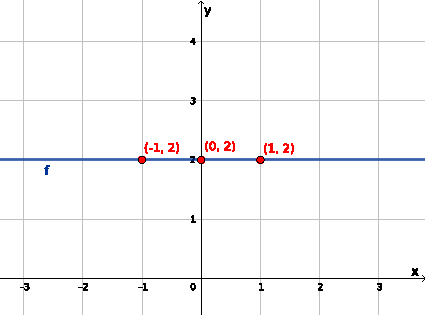
\includegraphics[width=7cm]{../Topicos/Figuras/f(x)=2.pdf}}
    \caption{Gráfico da função $f(x)=2$}
  \end{figure}

\subsection{Função identidade}

Dado um conjunto $A$ qualquer. A função $Id: A \rightarrow A$, definida por $Id(x)= x$ para todo $x \in A$ é chamada \textit{função identidade}.

Um exemplo de função identidade que vamos usar bastante é $Id: \R \rightarrow \R$ dada por $Id(x)= x$, cujo gráfico é:
\begin{figure}[H]
 \centering
    \fbox{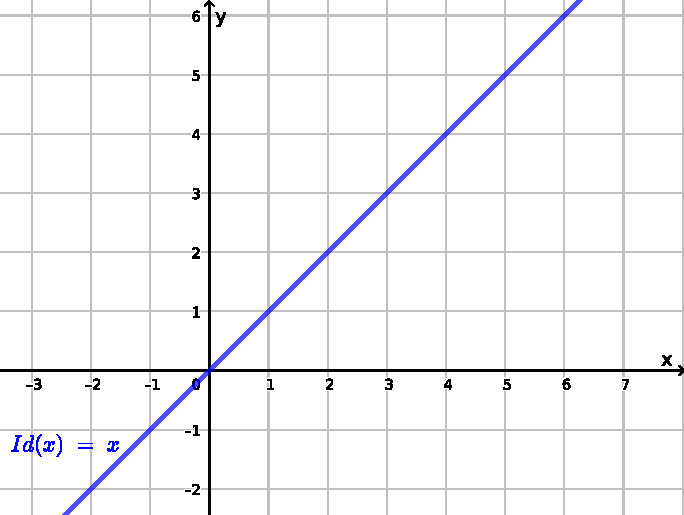
\includegraphics[width=7cm]{../Topicos/Figuras/Id(x)=x.pdf}}
    \caption{Gráfico da função $Id(x)=x$}
  \end{figure}

\subsection{Função inversa}

Considere uma função $f: A \rightarrow B$. Se existir uma função $g: B \rightarrow A$ tal que:
\[(g \circ f)(x)= x, \forall x \in A\]
\[ \text {e}\]
\[(f \circ g)(x)= x, \forall x \in B\]
então dizemos que $f$ é inversível e que $g$ é a inversa de $f$, ou seja, $g= f^{-1}$.

\begin{exem}
 A função $f: \R \rightarrow \R$ dada por $f(x)= x+2$ é injetora, e sobrejetora portanto, existe uma função $g: \R \rightarrow \R$ dada por $g(x)= x-2$, tal que:
 \[h(x)= (f \circ g)(x)= f(g(x))= (x-2) + 2= x-2+2= x \Rightarrow (f \circ g)(x)= Id(x)\]
 \[\text{e}\]
 \[(g \circ f)(x)= g(f(x))= (x+2) - 2= x+2-2= x \Rightarrow (g \circ f)(x)= Id(x) ,\]
 logo $g= f^{-1}$ é a função inversa de $f$.

 \begin{figure}[H]
 \centering
    \fbox{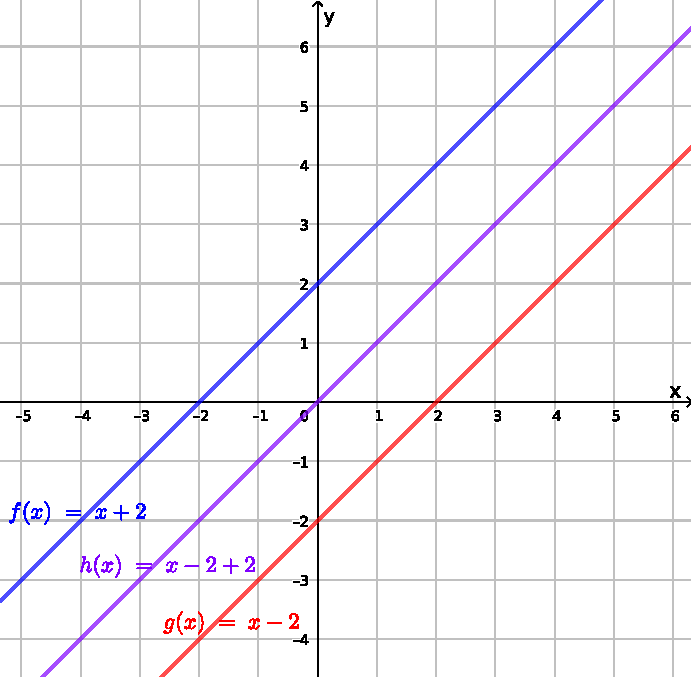
\includegraphics[width=8cm]{../Topicos/Figuras/funcao_composta.pdf}}
    \caption{Composta das funções $f$ e $g$}
  \end{figure}

\end{exem}


\subsection{Funções polinomiais de grau \texorpdfstring{$n$}{n}}

 São funções $f: \mathbb{R} \rightarrow \mathbb{R}$ com a seguinte regra geral:
 \[f(x) = a_0 + a_1 x + a_2 x^2 + a_3 x^3 + \cdots + a_n x^n\]
 onde $\{a_0, a_1, a_2, a_3, \ldots a_n\} \in \R$ com $a_n \neq 0$, $n \in \mathbb{N}$.

 Casos particulares:
 \begin{itemize}
 \item Funções do 1º grau, ou função afim

 São funções $f: \R \rightarrow \R$ dadas por:
 \[f(x)= ax + b\]
 {\color{red} zeros ou raízes, crescente, decrescente, gráfico, coeficiente angular e coeficiente linear}

 Os zeros ou raízes das funções de 1ª grau $f$ são os $x \in dom(f)$ tais que $ax+b=0$, como esta equação do 1º grau possui uma única raiz, a função de 1º grau também possui uma única raiz $x_1$, o ponto $(x_1, 0) \in \R^2$ é o ponto de interseção do gráfico da $f$ com o eixo $x$.

 Quando $\destaque{a > 0}$ temos que dados $x_1 < x_2 \in dom(f)$, teremos $f(x_1) < f(x_2)$, logo $f$ é por definição \textbf{crescente}.

 Quando $\destaque{a < 0}$ temos que dados $x_1 < x_2 \in dom(f)$, teremos $f(x_1) > f(x_2)$, logo $f$ é por definição \textbf{descrescente}.

 Na figura abaixo temos os gráficos de três funções de primeiro grau, sendo uma delas a função $f_1(x)= x$, que é a função identidade.
 \begin{figure}[H]
 \centering
    \fbox{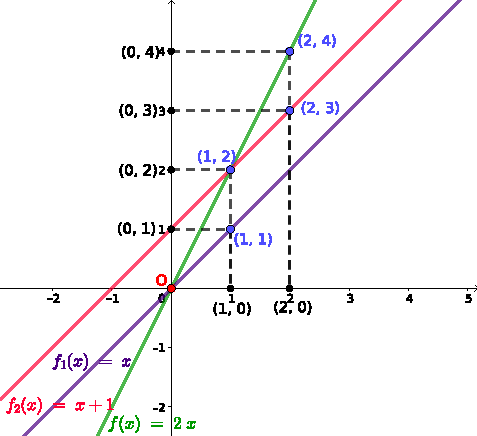
\includegraphics[width=8cm]{../Topicos/Figuras/funcao1grau.pdf}}
    \caption{Gráficos de funções do 1º grau}
  \end{figure}



 \item Funções do 2º grau ou função quadrática

 São funções $f: \R \rightarrow \R$ dadas por:
 \[f(x)= ax^2 + bx + c\]
 {\color{red} zeros ou raízes, concavidade, máximos ou mínimo}

 Os zeros ou raízes das funções de 2º grau $f$, quando existem, são os $x \in dom(f)$ tais que $ax^2+bx+c=0$. Por ser esta uma equação do 2º grau temos três situações a considerar, dependendo do valor de $\Delta$:
 \[\destaque{\Delta= b^2 - 4*a*c}\]
 Se $\destaque{\Delta < 0}$ a função $f$ não possui raízes reais;

 Se $\destaque{\Delta = 0}$ a função $f$ possui uma única raiz real;

 Se $\destaque{\Delta > 0}$ a função $f$ possui duas raízes reais distintas, que podem ser calculadas resolvendo a equação de 2º grau através da fórmula para equações de 2º grau.

 Com relação a concavidade, o gráfico da função de 2º grau tem concavidade voltada \textbf{para cima} quando $\destaque{a > 0}$, e concavidade voltada \textbf{para baixo} quando $\destaque{a < 0}$.

 Em ambos os casos a função do 2º grau possui um vértice dado pela seguinte equação:

 \[ \destaque{V= \left(\frac{- b}{2a}, \frac{- \Delta}{4a} \right)} .\]

 No caso em que $a > 0$, o vértice do gráfico da função de 2º grau é um ponto de mínimo da função.

 No caso em que $a < 0$, o vértice do gráfico da função de 2º grau é um ponto de máximo da função.


  \begin{figure}[H]
   \fbox{\subfigure[$a > 0$ e $\Delta < 0$]{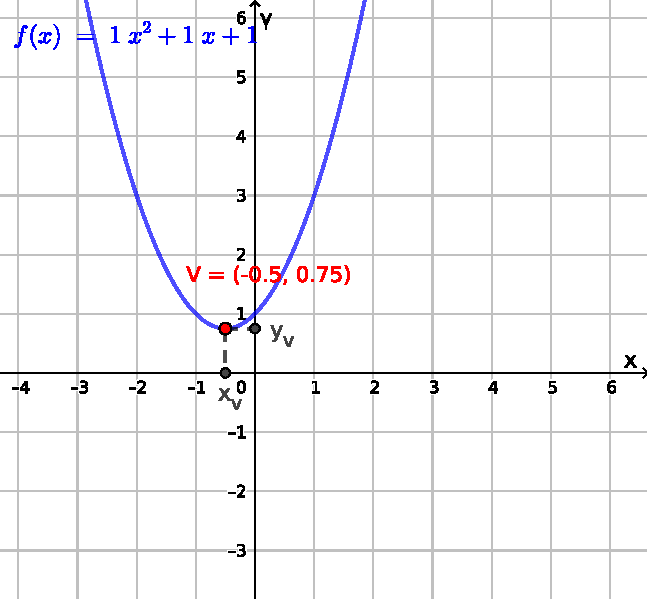
\includegraphics[width=7cm,height=6cm]{../Topicos/Figuras/f1.pdf}}}
   \fbox{\subfigure[$a > 0$ e $\Delta = 0$]{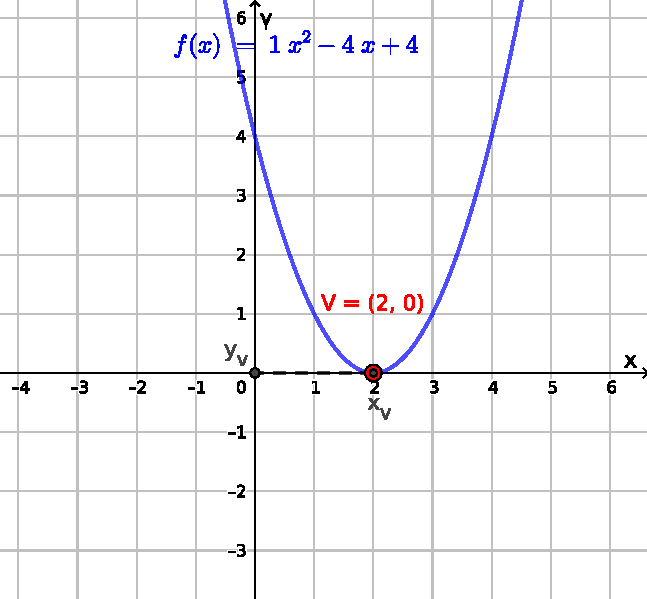
\includegraphics[width=7cm,height=6cm]{../Topicos/Figuras/f2.pdf}}}
   \fbox{\subfigure[$a > 0$ e $\Delta > 0$]{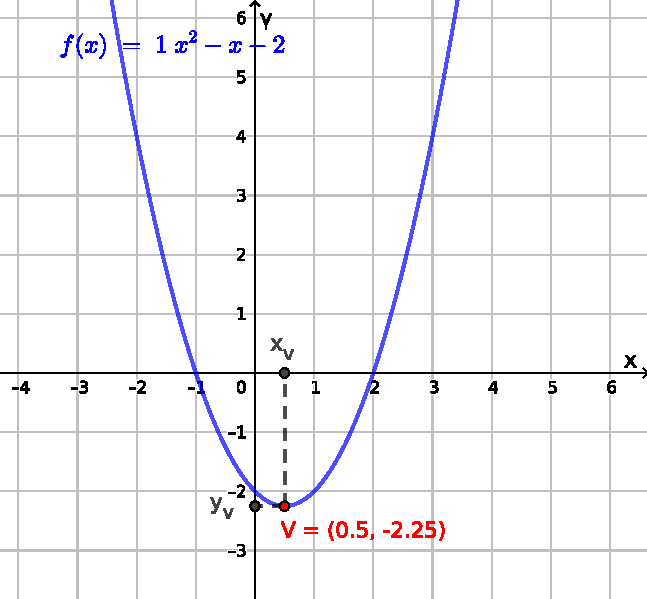
\includegraphics[width=7cm,height=6cm]{../Topicos/Figuras/f3.pdf}}}
   \fbox{\subfigure[$a < 0$ e $\Delta < 0$]{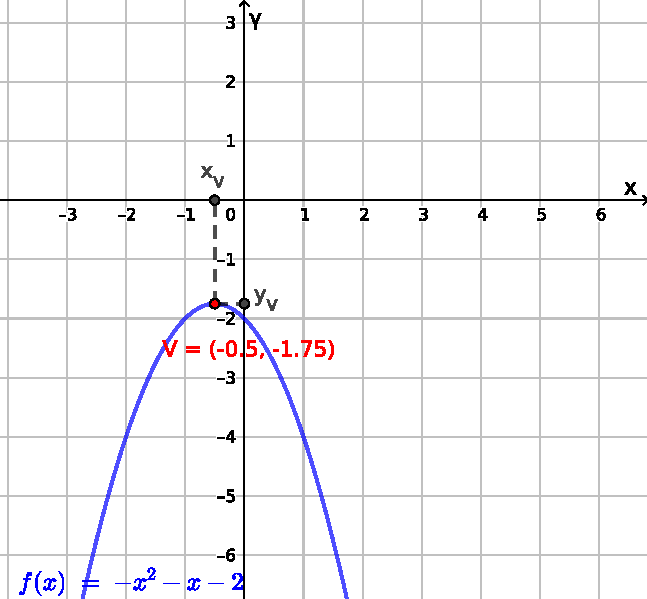
\includegraphics[width=7cm,height=6cm]{../Topicos/Figuras/f4.pdf}}}
   \fbox{\subfigure[$a < 0$ e $\Delta = 0$]{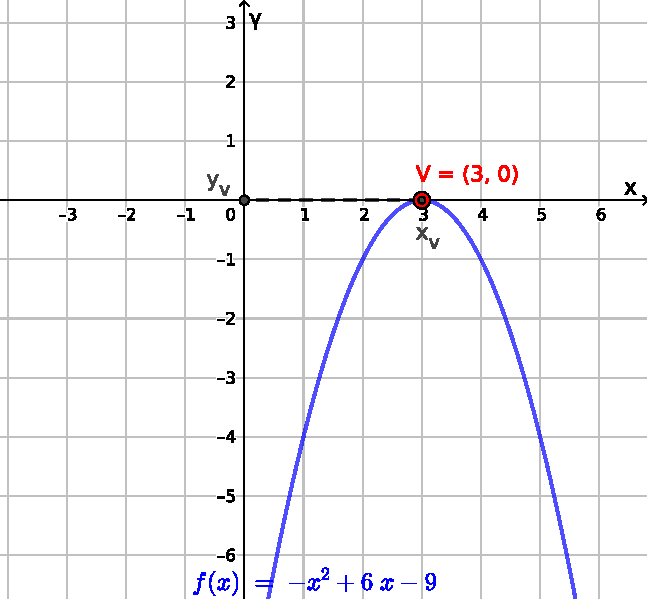
\includegraphics[width=7cm,height=6cm]{../Topicos/Figuras/f5.pdf}}}
   \fbox{\subfigure[$a < 0$ e $\Delta > 0$]{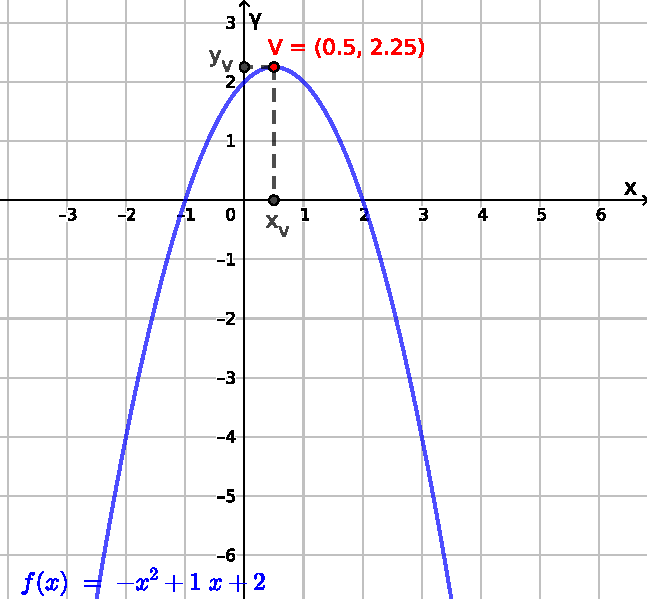
\includegraphics[width=7cm,height=6cm]{../Topicos/Figuras/f6.pdf}}}
   \caption{Gráficos de funções do 2º grau}
\end{figure}

  \newpage
 \item Funções do 3º grau ou função cúbica

 São funções $f: \R \rightarrow \R$ dadas por:
 \[f(x)= ax^3 + bx^2 + cx + d .\]
 {\color{red} zeros ou raízes, concavidades, máximos local ou mínimo local}

 As raízes ou zeros das funções de 3º grau são os $x \in \R$ tais que $ax^3 + bx^2 + cx + d=0$. Assim as função de 3º grau podem classificadas de acordo com suas raízes em 4 casos:
 \begin{enumerate}[(I)]
  \item 3 raízes distintas;
  \item 1 única raiz;
  \item 3 raízes sendo duas delas iguais;
  \item 3 raízes iguais.
 \end{enumerate}
 Estes casos estão representados nos gráficos abaixo, onde consideramos sempre $a< 0$, o caso $a> 0$ é análogo.


   \begin{figure}[H]
   \fbox{\subfigure[$a < 0$]{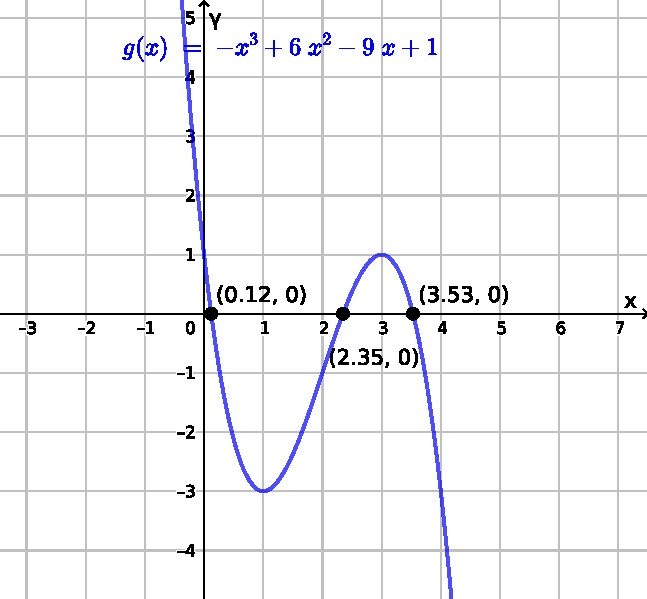
\includegraphics[width=7cm,height=6cm]{../Topicos/Figuras/g1.pdf}}}
   \fbox{\subfigure[$a < 0$]{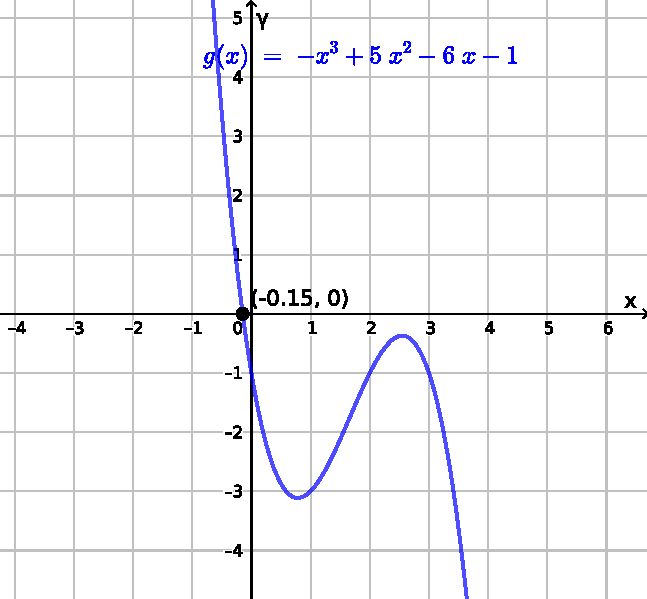
\includegraphics[width=7cm,height=6cm]{../Topicos/Figuras/g2.pdf}}}
   \fbox{\subfigure[$a < 0$]{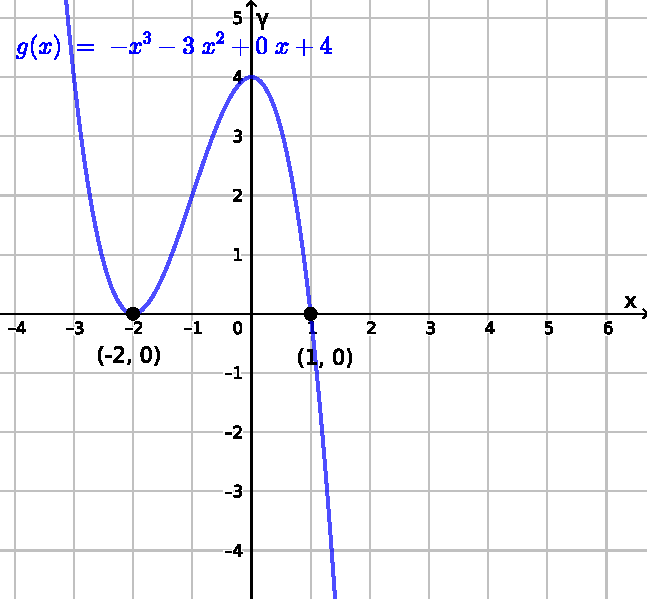
\includegraphics[width=7cm,height=6cm]{../Topicos/Figuras/g3.pdf}}}
   \fbox{\subfigure[$a < 0$]{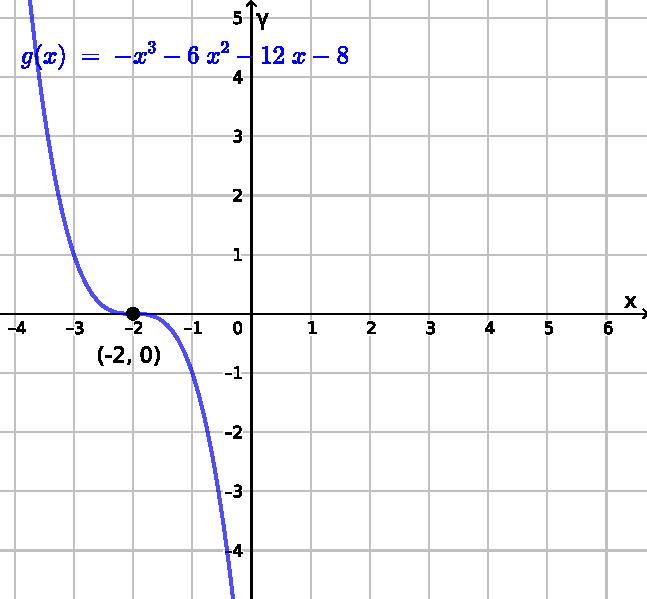
\includegraphics[width=7cm,height=6cm]{../Topicos/Figuras/g4.pdf}}}
   \caption{Gráficos de funções do 3º grau}
  \end{figure}

 Observamos que as funções cúbicas não possuem pontos de mínimo e máximo global, estas possuem apenas pontos extremantes locais. Além disso o estudo de suas concavidades pode ser feito apenas localmente.

 \end{itemize}

  \subsection{Função modular}

  \[f(x)= |x| = \begin{cases}
                 x, \text{ se } x \geq 0 \\
                 -x, \text{ se } x \leq 0
                \end{cases}\]

  \section{Funções Trigonométricas}

  Casos particulares:

  {\color{red} períodos, amplitude, intervalo de bijetividade, função inversa}

  \begin{itemize}
  \item Função Seno: $f(x)= sen (x)$

  \frame{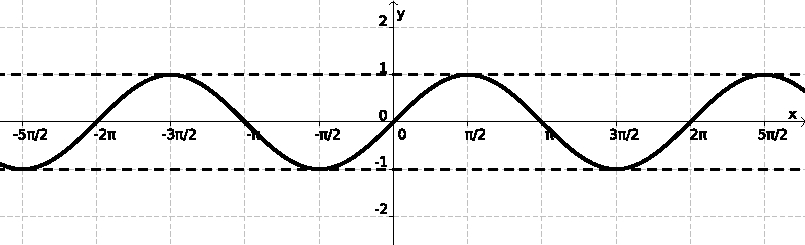
\includegraphics[width=12.0cm]{../Topicos/Figuras/sen.pdf}}

  \item Função Cosseno: $f(x)= cos (x)$

  \frame{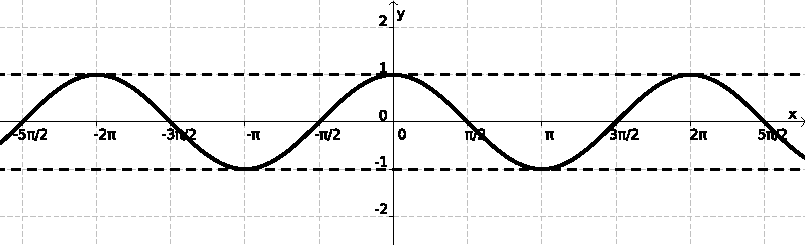
\includegraphics[width=12.0cm]{../Topicos/Figuras/cos.pdf}}

  \item Função Tangente: $f(x)= tan (x)$

  \frame{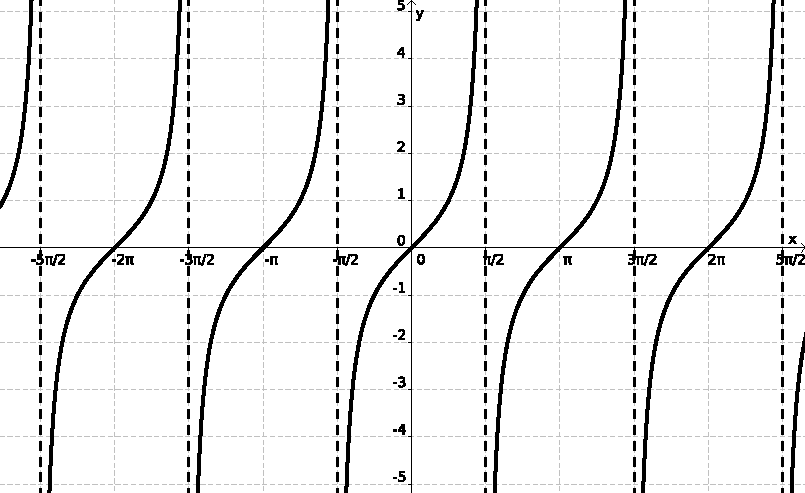
\includegraphics[width=12.0cm]{../Topicos/Figuras/tan.pdf}}

  \item Função Cossecante: $csc(x)= \dfrac{1}{sen (x)}$

  \frame{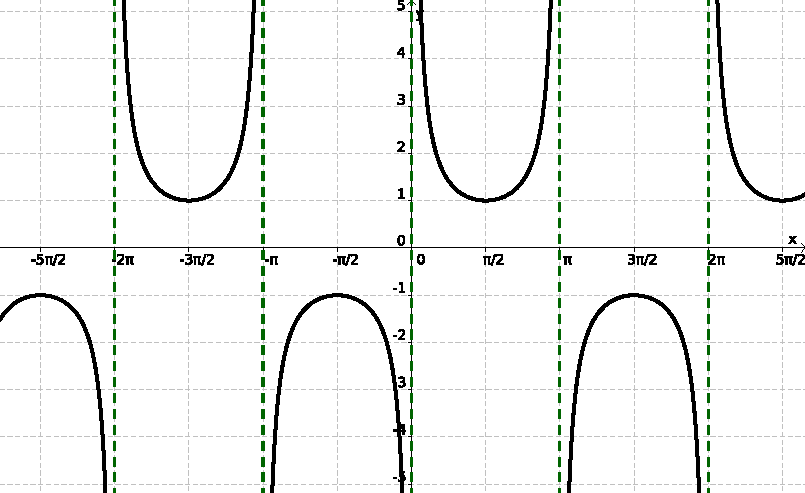
\includegraphics[width=12.0cm]{../Topicos/Figuras/csc.pdf}}

  \item Função Secante: $sec(x)= \dfrac{1}{cos (x)}$

  \frame{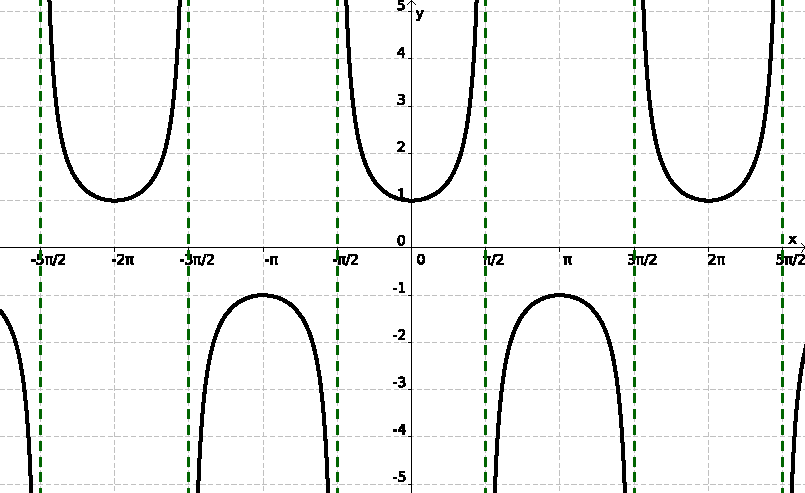
\includegraphics[width=12.0cm]{../Topicos/Figuras/sec.pdf}}

  \item Função Cotangente: $cot(x)= \dfrac{1}{tan (x)}$

  \frame{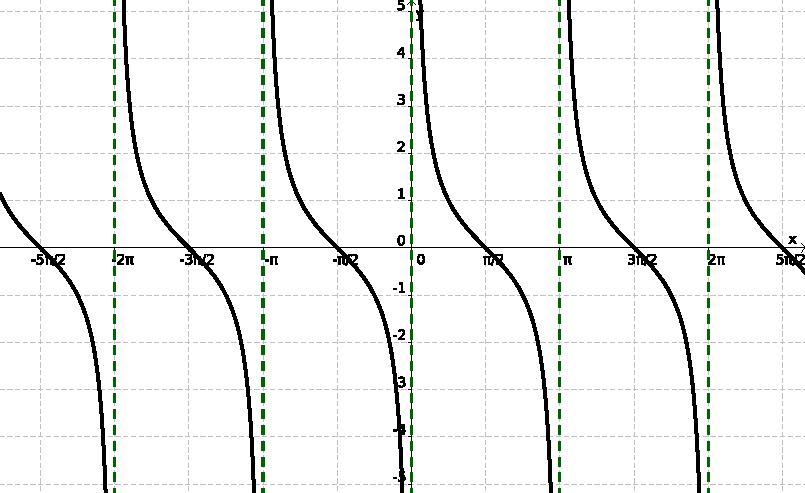
\includegraphics[width=12.0cm]{../Topicos/Figuras/cot.pdf}}

  \textbf{Funções Inversas}
  \item Função Arco Seno: $sen^{-1}(x)= arcsen (x)$

  \frame{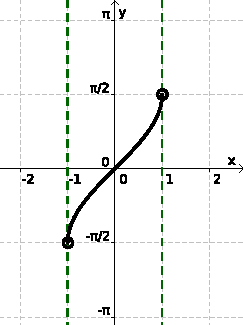
\includegraphics[width=5.0cm]{../Topicos/Figuras/arcsen.pdf}}

  \item Função Arco Cosseno: $cos^{-1}(x)= arccos (x)$

  \frame{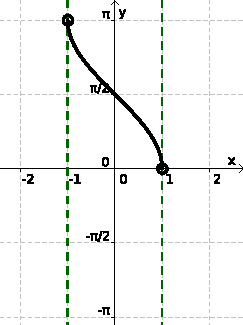
\includegraphics[width=5.0cm]{../Topicos/Figuras/arccos.pdf}}

  \item Função Arco Tangente: $tan^{-1}(x)= arctan (x)$

  \frame{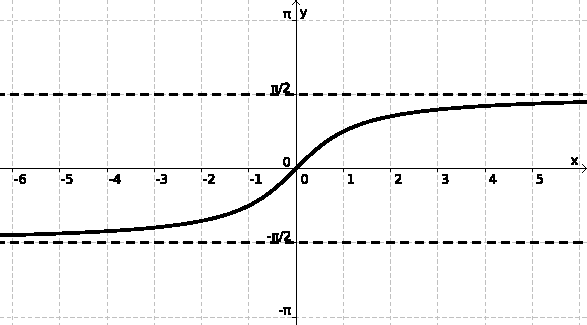
\includegraphics[width=12.0cm]{../Topicos/Figuras/arctan.pdf}}

  \end{itemize}

 \subsection{Funções exponenciais}

 São funções $f: \mathbb{R} \rightarrow \mathbb{R_{+}^{*}} $ tais que:
 \[f(x) = a^x\]
 onde é dado $a \in \mathbb{R_{+}}$ satisfazendo $0 < a$ e $a \neq 1$. Estas funções são chamadas funções exponenciais de base $a$.

 Se $0 < a < 1$ a função $f$ é decrescente. Se $1 < a < +\infty$ a função $f$ é crescente.

 \begin{figure}[H]
   \fbox{\subfigure[$0 < a < 1$ ]{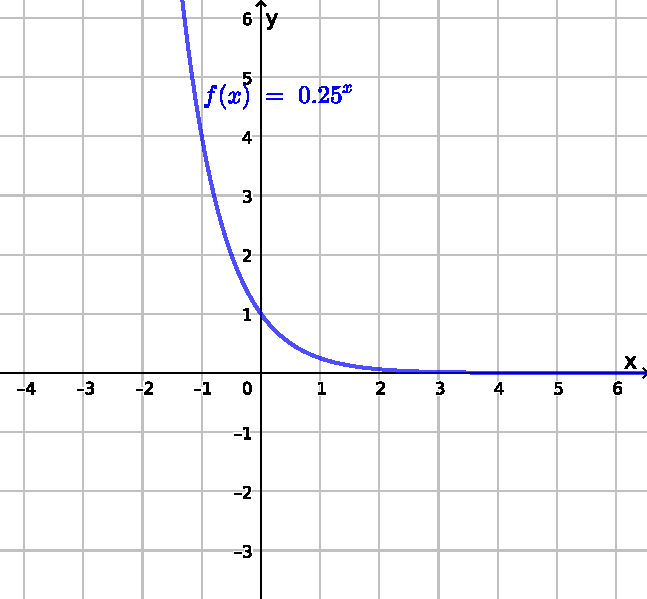
\includegraphics[width=7cm,height=6cm]{../Topicos/Figuras/e1.pdf}}}
   \fbox{\subfigure[$1 < a < +\infty$]{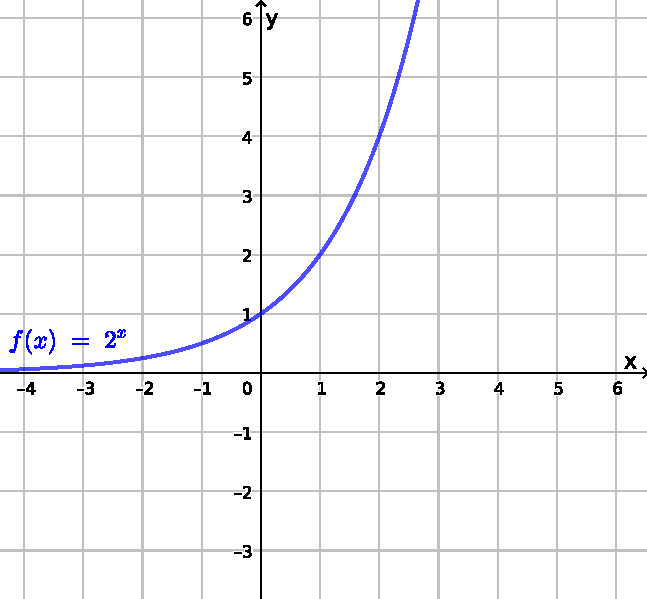
\includegraphics[width=7cm,height=6cm]{../Topicos/Figuras/e2.pdf}}}
   \caption{Gráficos de funções exponenciais}
  \end{figure}

  Um caso especial de função exponencial é quando $a= e$, assim $f: \mathbb{R} \rightarrow \mathbb{R_{+}^{*}} $ será dada por:
  \[f(x) = e^x\]
  esta função é uma função crescente, e seu gráfico é:

  \begin{figure}[H]
 \centering
    \fbox{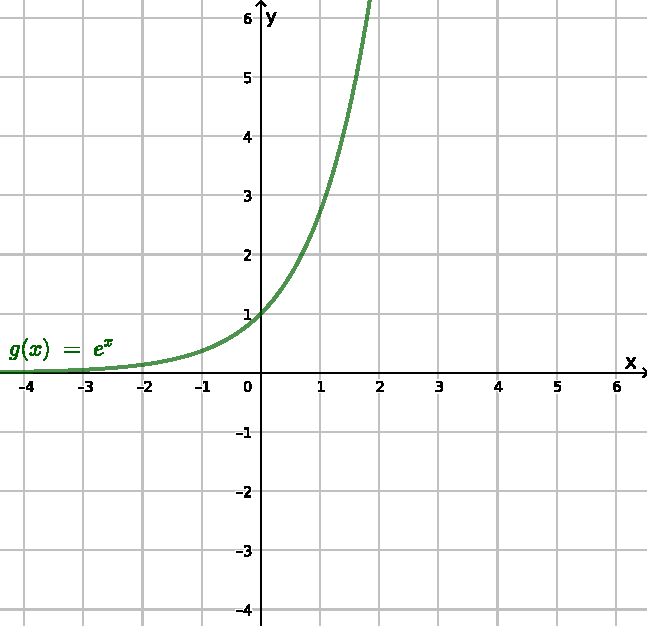
\includegraphics[width=7cm]{../Topicos/Figuras/exponencial.pdf}}
    \caption{Gráficos da função exponencial}
  \end{figure}

 Sejam $a > 0$, $b > 0$, $x$ e $y$ reais quaisquer, as seguintes propriedades são satisfeitas:
 \begin{enumerate}
  \item $a^x a^y= a^{x+y}$;
  \item $(a^x)^y= a^{xy}$;
  \item $(ab)^x= a^x b^x$;
  \item Se $a > 1$ e $x < y$, então $a^x < a^y$;
  \item Se $0 < a < 1$ e $x < y$, então $a^x > a^y$.
 \end{enumerate}

 De (4) obtemos que $f(x)= a^x$, $a > 1$, é estritamente crescente em $\R$. De (5) obtemos que $f(x)= a^x$, $0 < a < 1$, é estritamente decrescente em $\R$. Portanto $\forall a > 0$ e $a \neq 1$ temos que a função exponencial $f(x)= a^x$ é bijetora.


 \subsection{Funções logarítmicas}

 São funções $f: \mathbb{R_{+}^{*}} \rightarrow \mathbb{R} $ tais que:
 \[f(x) = \log_{a}(x)\]
 onde é dado $a \in \mathbb{R}$ satisfazendo $0 < a$ e $a \neq 1$. Estas funções são denominadas funções logarítmicas de base $a$.

 Observemos que dado um número real $a> 0$ e $a \neq 1$, para cada $y>0$ existe um único número real $x$ tal que $a^x= y$, já que como visto anteriormente a função exponencial $f(x)= a^x$ é bijetiva. Podemos assim definir o logaritmo de $y$ na base $a$ como sendo o número real $x$ tal que $a^x= y$. Simbolicamente,
 \[\destaque{\log_a(y)= x  \Leftrightarrow a^x= y}.\]

 Portanto, as funções logarítmica e exponencial são inversas uma da outra.

 Se $0 < a < 1$ a função $f$ é decrescente. Se $1 < a < +\infty$ a função $f$ é crescente.

 \begin{figure}[H]
   \fbox{\subfigure[$0 < a < 1$ ]{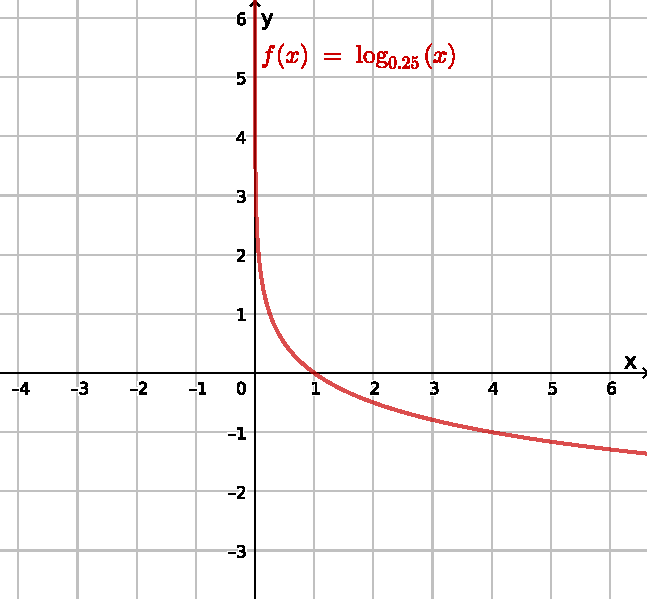
\includegraphics[width=7cm,height=6cm]{../Topicos/Figuras/l1.pdf}}}
   \fbox{\subfigure[$1 < a < +\infty$]{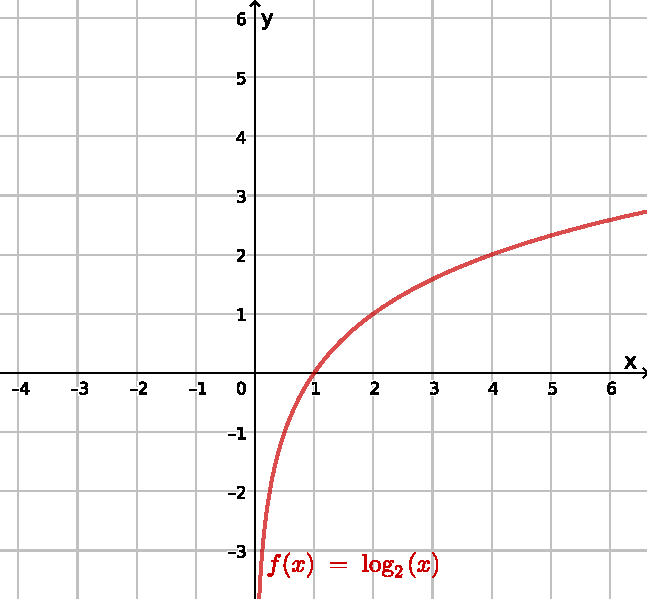
\includegraphics[width=7cm,height=6cm]{../Topicos/Figuras/l2.pdf}}}
   \caption{Gráficos de funções logarítmicas}
  \end{figure}

 Um caso especial de função logarítmica é quando $a= e$, assim $f: \mathbb{R_{+}^{*}} \rightarrow \mathbb{R} $ será dada por:
  \[f(x) = \log_{e}(x)= ln(x)\]
 esta função é chamada logaritmo neperiano, que é uma função crescente, e seu gráfico é:

  \begin{figure}[H]
 \centering
    \fbox{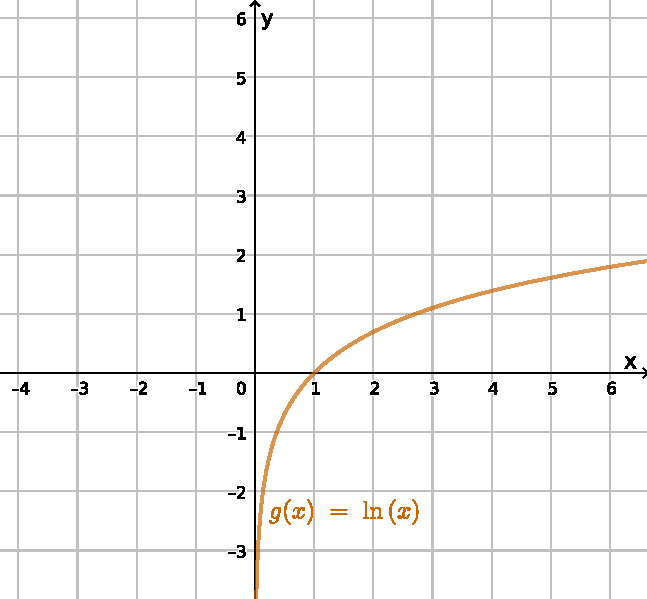
\includegraphics[width=7cm]{../Topicos/Figuras/logaritmo.pdf}}
    \caption{Gráficos da função logaritmo neperiano}
  \end{figure}

  Sejam $a> 0$, $a \neq 1$, $b> 0$, $b \neq 1$, $\alpha > 0$, $\beta > 0$ reais quaisquer. São válidas as seguintes propriedades:
  \begin{enumerate}
   \item $\log_{a}(\alpha\beta)=\log_{a}(\alpha) + \log_{a}(\beta)$;
   \item $\log_{a}(\alpha)^{\beta}=\log_{a}\beta(\alpha)$;
   \item $\log_{a}\frac{\alpha}{\beta}=\log_{a}(\alpha) - \log_{a}(\beta)$;
   \item (Mudança de base) \[\log_{a}(\alpha)=\frac{\log_{b}(\alpha)}{\log_{b}(a)};\]
   \item Se $a> 1$ e $\alpha < \beta$, então $\log_{a}(\alpha) < \log_{a}(\beta)$;
   \item Se $0 < a < 1$ e $\alpha < \beta$, então $\log_{a}(\alpha) > \log_{a}(\beta)$;
  \end{enumerate}

 \newpage
